\documentclass{article}
\usepackage{graphicx}
\graphicspath{ {../figures/} }
\title{exploratory data analysis}
\author{Telegin Konstantin and Zakirova Svetlana}
\date{May 2017}
\begin{document}
	\maketitle
		
	we have compared suppliers by three ways. Nothing of it doesn't include some result in numeric value. All conclusions was reached by plots. In our cases it contain quite enought information. 

	
	\section{First way}
The first what comes to mind is to compare how many sword produce both suppliers and how many from it was broken in absolute and relative values.\\
	calculations present following results:\\

supplier: harpy.co\\
   produced: 31532\\
   broken: 6080 (19.28\%)\\

supplier: westeros.inc\\
   produced: 31625\\
   broken: 8268 (26.14\%)\\
	
	As we can see, both suppliers make about equal numbers of swords. But westeros'es have more defect sword, so it supply less proper sword us. Moreover, we think that soldier would prefer to have not any weapon instead of to have sword which will brake right in battle. So we can conclude, that in this terms westeros.inc is better.
	\
	
	\section{Second way}
	
	Besides overall number of swords we must distinguish it various days. obciuosly, sword made in first better than it made in last day. So we calculate how many swords both suppliers had been made by each day without defect. 
   
   \hbox{\hspace{-5em} 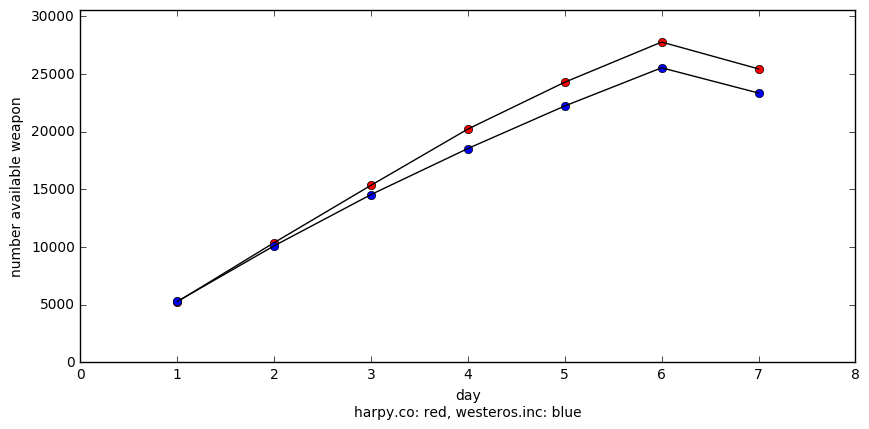
\includegraphics[scale=0.7]{daily_analyze}}

	If sword brake in some day it is not counted in this way.
	As we can see, harpy make available more swords every day. So in this case harpy is better.
	
	
	\section{Third way}
	
	As we have mentioned before, defects is bad not only because it decrease available weapons number, but it make some suspense. It's badly when your sword brake during the battle. So let's calculate how much defects swords have both companies for each day.
	
   \hbox{\hspace{-5em} 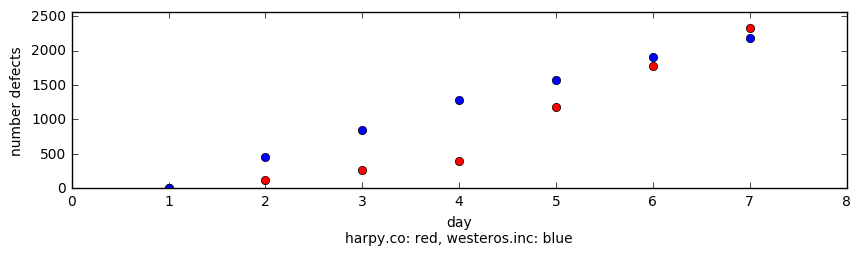
\includegraphics[scale=0.7]{daily_defects}}
		
	So, westeros has low-quality steel. Especialy it appers in firsts days, that is bad too.
	Calculate for each day part of defects swords to the number of swords available to the begin of the day, i.e. including swords which will be broken.
	\hbox{\hspace{-5em} 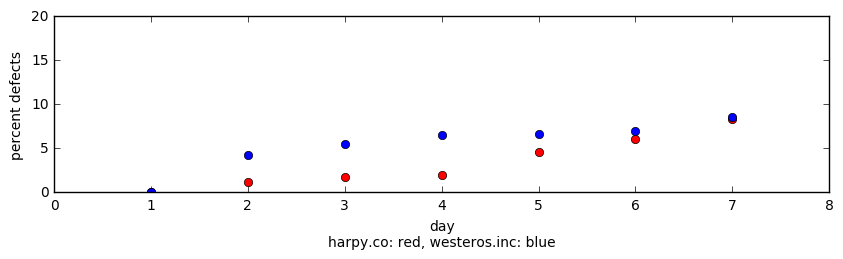
\includegraphics[scale=0.7]{daily_defects_percent}}
			
	\section{Conclusion}	
	We have made several simple comparsion between companies. And harpy is better in all this case - it make more swords and more durable.
	
	
\end{document}